% Name: Pentagon equation
% Description: The five bracketings of four objects on a regular pentagon, joined by the associator F: both routes from ((ab)c)d to a(b(cd)) agree.
% Tags: pentagon equation, F-move, associator, coherence

\usetikzlibrary{arrows.meta}

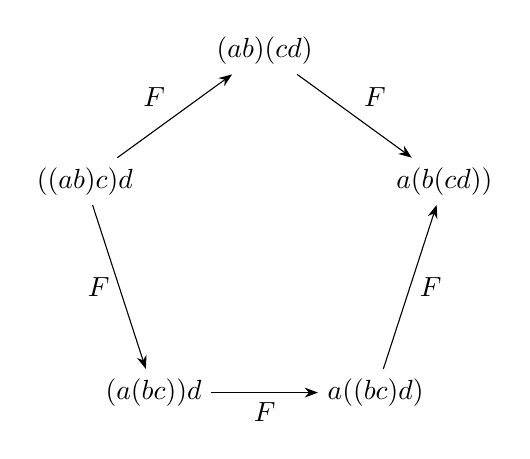
\begin{tikzpicture}[>={Stealth}]
  \node (A) at (162:2.4) {$((ab)c)d$};
  \node (B) at (90:2.4)  {$(ab)(cd)$};
  \node (C) at (18:2.4)  {$a(b(cd))$};
  \node (D) at (234:2.4) {$(a(bc))d$};
  \node (E) at (306:2.4) {$a((bc)d)$};
  \draw[->] (A) -- node[above left]  {$F$} (B);
  \draw[->] (B) -- node[above right] {$F$} (C);
  \draw[->] (A) -- node[left]        {$F$} (D);
  \draw[->] (D) -- node[below]       {$F$} (E);
  \draw[->] (E) -- node[right]       {$F$} (C);
\end{tikzpicture}
